% Coordinator-owned insertion: copy the final PDF to canonical figures/ first.
\begin{figure}[htbp]
\centering
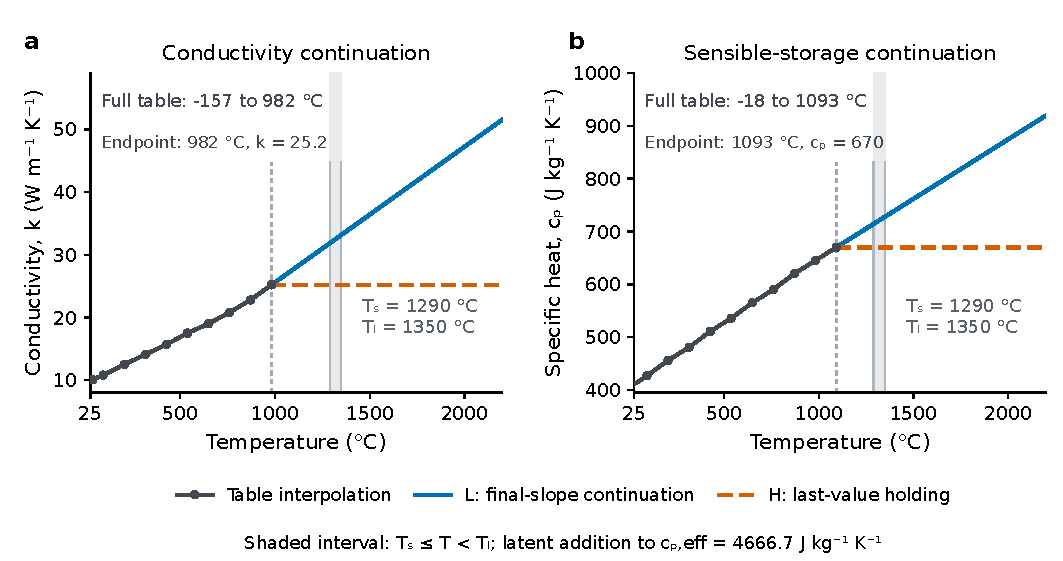
\includegraphics[width=\textwidth]{figures/ammt-property-continuations.pdf}
\caption{Actual IN625 property inputs and the two continuation choices. (a) Conductivity and (b) sensible specific heat use the knots loaded by the executed material routine, with common piecewise-linear interpolation below the respective endpoints. The final knots are 982~$^\circ$C and 25.2~\si{\watt\per\metre\per\kelvin} for $k$, and 1093~$^\circ$C and 670~\si{\joule\per\kilogram\per\kelvin} for $c_p$. L continues the final tabulated secant; H holds the final value. The displayed window is 25--2200~$^\circ$C; all 15 conductivity and 12 specific-heat source rows, including those below 25~$^\circ$C, are retained in the accompanying data and used in interpolation. Shading marks the adopted 1290--1350~$^\circ$C phase interval. The latent addition to effective specific heat within this interval is 4666.7~\si{\joule\per\kilogram\per\kelvin} and is stated separately from sensible $c_p$. The supplier describes conductivity as measured and specific heat as calculated typical alloy data~\cite{specialmetals625}; the plotted high-temperature continuations are modeling choices.}
\label{fig:properties}
\end{figure}

% Suggested uptake at the material-table paragraph:
% Figure~\ref{fig:properties} shows that both data endpoints lie below the adopted solidus, so the phase-changing region depends on the continuation rules examined in the fixed-source contrast.
